\documentclass[1p]{elsarticle_modified}
%\bibliographystyle{elsarticle-num}

%\usepackage[colorlinks]{hyperref}
%\usepackage{abbrmath_seonhwa} %\Abb, \Ascr, \Acal ,\Abf, \Afrak
\usepackage{amsfonts}
\usepackage{amssymb}
\usepackage{amsmath}
\usepackage{amsthm}
\usepackage{scalefnt}
\usepackage{amsbsy}
\usepackage{kotex}
\usepackage{caption}
\usepackage{subfig}
\usepackage{color}
\usepackage{graphicx}
\usepackage{xcolor} %% white, black, red, green, blue, cyan, magenta, yellow
\usepackage{float}
\usepackage{setspace}
\usepackage{hyperref}

\usepackage{tikz}
\usetikzlibrary{arrows}

\usepackage{multirow}
\usepackage{array} % fixed length table
\usepackage{hhline}

%%%%%%%%%%%%%%%%%%%%%
\makeatletter
\renewcommand*\env@matrix[1][\arraystretch]{%
	\edef\arraystretch{#1}%
	\hskip -\arraycolsep
	\let\@ifnextchar\new@ifnextchar
	\array{*\c@MaxMatrixCols c}}
\makeatother %https://tex.stackexchange.com/questions/14071/how-can-i-increase-the-line-spacing-in-a-matrix
%%%%%%%%%%%%%%%

\usepackage[normalem]{ulem}

\newcommand{\msout}[1]{\ifmmode\text{\sout{\ensuremath{#1}}}\else\sout{#1}\fi}
%SOURCE: \msout is \stkout macro in https://tex.stackexchange.com/questions/20609/strikeout-in-math-mode

\newcommand{\cancel}[1]{
	\ifmmode
	{\color{red}\msout{#1}}
	\else
	{\color{red}\sout{#1}}
	\fi
}

\newcommand{\add}[1]{
	{\color{blue}\uwave{#1}}
}

\newcommand{\replace}[2]{
	\ifmmode
	{\color{red}\msout{#1}}{\color{blue}\uwave{#2}}
	\else
	{\color{red}\sout{#1}}{\color{blue}\uwave{#2}}
	\fi
}

\newcommand{\Sol}{\mathcal{S}} %segment
\newcommand{\D}{D} %diagram
\newcommand{\A}{\mathcal{A}} %arc


%%%%%%%%%%%%%%%%%%%%%%%%%%%%%5 test

\def\sl{\operatorname{\textup{SL}}(2,\Cbb)}
\def\psl{\operatorname{\textup{PSL}}(2,\Cbb)}
\def\quan{\mkern 1mu \triangleright \mkern 1mu}

\theoremstyle{definition}
\newtheorem{thm}{Theorem}[section]
\newtheorem{prop}[thm]{Proposition}
\newtheorem{lem}[thm]{Lemma}
\newtheorem{ques}[thm]{Question}
\newtheorem{cor}[thm]{Corollary}
\newtheorem{defn}[thm]{Definition}
\newtheorem{exam}[thm]{Example}
\newtheorem{rmk}[thm]{Remark}
\newtheorem{alg}[thm]{Algorithm}

\newcommand{\I}{\sqrt{-1}}
\begin{document}

%\begin{frontmatter}
%
%\title{Boundary parabolic representations of knots up to 8 crossings}
%
%%% Group authors per affiliation:
%\author{Yunhi Cho} 
%\address{Department of Mathematics, University of Seoul, Seoul, Korea}
%\ead{yhcho@uos.ac.kr}
%
%
%\author{Seonhwa Kim} %\fnref{s_kim}}
%\address{Center for Geometry and Physics, Institute for Basic Science, Pohang, 37673, Korea}
%\ead{ryeona17@ibs.re.kr}
%
%\author{Hyuk Kim}
%\address{Department of Mathematical Sciences, Seoul National University, Seoul 08826, Korea}
%\ead{hyukkim@snu.ac.kr}
%
%\author{Seokbeom Yoon}
%\address{Department of Mathematical Sciences, Seoul National University, Seoul, 08826,  Korea}
%\ead{sbyoon15@snu.ac.kr}
%
%\begin{abstract}
%We find all boundary parabolic representation of knots up to 8 crossings.
%
%\end{abstract}
%\begin{keyword}
%    \MSC[2010] 57M25 
%\end{keyword}
%
%\end{frontmatter}

%\linenumbers
%\tableofcontents
%
\newcommand\colored[1]{\textcolor{white}{\rule[-0.35ex]{0.8em}{1.4ex}}\kern-0.8em\color{red} #1}%
%\newcommand\colored[1]{\textcolor{white}{ #1}\kern-2.17ex	\textcolor{white}{ #1}\kern-1.81ex	\textcolor{white}{ #1}\kern-2.15ex\color{red}#1	}

{\Large $\underline{12n_{0296}~(K12n_{0296})}$}

\setlength{\tabcolsep}{10pt}
\renewcommand{\arraystretch}{1.6}
\vspace{1cm}\begin{tabular}{m{100pt}>{\centering\arraybackslash}m{274pt}}
\multirow{5}{120pt}{
	\centering
	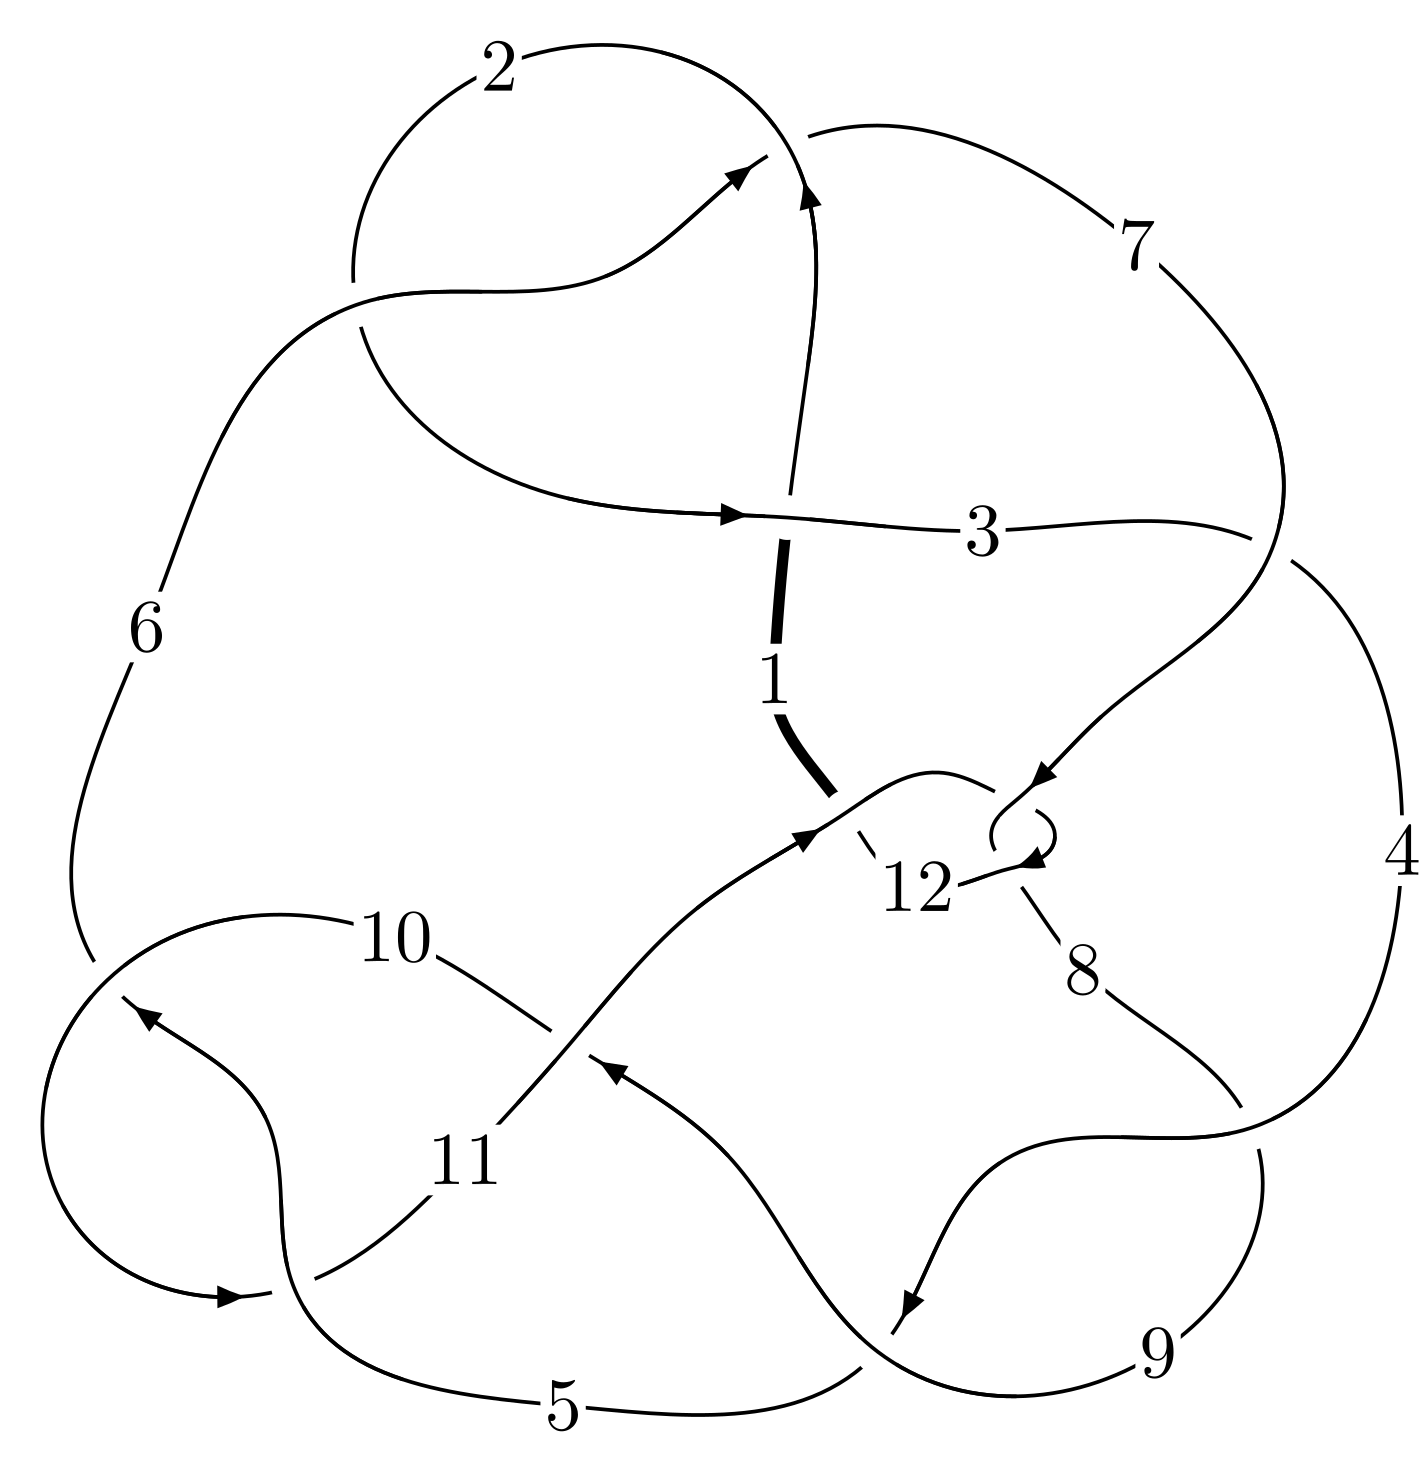
\includegraphics[width=112pt]{../../../GIT/diagram.site/Diagrams/png/2385_12n_0296.png}\\
\ \ \ A knot diagram\footnotemark}&
\allowdisplaybreaks
\textbf{Linearized knot diagam} \\
\cline{2-2}
 &
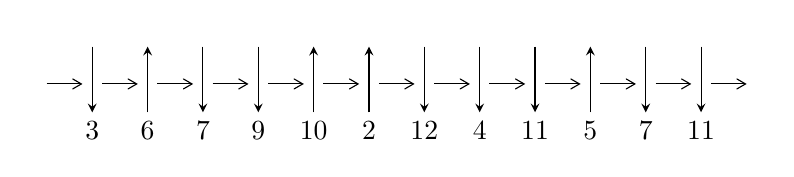
\begin{tikzpicture}[x=20pt, y=17pt]
	% nodes
	\node (C0) at (0, 0) {};
	\node (C1) at (1, 0) {};
	\node (C1U) at (1, +1) {};
	\node (C1D) at (1, -1) {3};

	\node (C2) at (2, 0) {};
	\node (C2U) at (2, +1) {};
	\node (C2D) at (2, -1) {6};

	\node (C3) at (3, 0) {};
	\node (C3U) at (3, +1) {};
	\node (C3D) at (3, -1) {7};

	\node (C4) at (4, 0) {};
	\node (C4U) at (4, +1) {};
	\node (C4D) at (4, -1) {9};

	\node (C5) at (5, 0) {};
	\node (C5U) at (5, +1) {};
	\node (C5D) at (5, -1) {10};

	\node (C6) at (6, 0) {};
	\node (C6U) at (6, +1) {};
	\node (C6D) at (6, -1) {2};

	\node (C7) at (7, 0) {};
	\node (C7U) at (7, +1) {};
	\node (C7D) at (7, -1) {12};

	\node (C8) at (8, 0) {};
	\node (C8U) at (8, +1) {};
	\node (C8D) at (8, -1) {4};

	\node (C9) at (9, 0) {};
	\node (C9U) at (9, +1) {};
	\node (C9D) at (9, -1) {11};

	\node (C10) at (10, 0) {};
	\node (C10U) at (10, +1) {};
	\node (C10D) at (10, -1) {5};

	\node (C11) at (11, 0) {};
	\node (C11U) at (11, +1) {};
	\node (C11D) at (11, -1) {7};

	\node (C12) at (12, 0) {};
	\node (C12U) at (12, +1) {};
	\node (C12D) at (12, -1) {11};
	\node (C13) at (13, 0) {};

	% arrows
	\draw[->,>={angle 60}]
	(C0) edge (C1) (C1) edge (C2) (C2) edge (C3) (C3) edge (C4) (C4) edge (C5) (C5) edge (C6) (C6) edge (C7) (C7) edge (C8) (C8) edge (C9) (C9) edge (C10) (C10) edge (C11) (C11) edge (C12) (C12) edge (C13) ;	\draw[->,>=stealth]
	(C1U) edge (C1D) (C2D) edge (C2U) (C3U) edge (C3D) (C4U) edge (C4D) (C5D) edge (C5U) (C6D) edge (C6U) (C7U) edge (C7D) (C8U) edge (C8D) (C9U) edge (C9D) (C10D) edge (C10U) (C11U) edge (C11D) (C12U) edge (C12D) ;
	\end{tikzpicture} \\
\hhline{~~} \\& 
\textbf{Solving Sequence} \\ \cline{2-2} 
 &
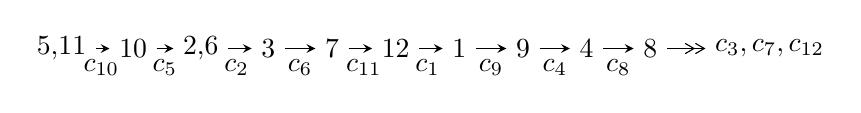
\begin{tikzpicture}[x=23pt, y=7pt]
	% node
	\node (A0) at (-1/8, 0) {5,11};
	\node (A1) at (1, 0) {10};
	\node (A2) at (33/16, 0) {2,6};
	\node (A3) at (25/8, 0) {3};
	\node (A4) at (33/8, 0) {7};
	\node (A5) at (41/8, 0) {12};
	\node (A6) at (49/8, 0) {1};
	\node (A7) at (57/8, 0) {9};
	\node (A8) at (65/8, 0) {4};
	\node (A9) at (73/8, 0) {8};
	\node (C1) at (1/2, -1) {$c_{10}$};
	\node (C2) at (3/2, -1) {$c_{5}$};
	\node (C3) at (21/8, -1) {$c_{2}$};
	\node (C4) at (29/8, -1) {$c_{6}$};
	\node (C5) at (37/8, -1) {$c_{11}$};
	\node (C6) at (45/8, -1) {$c_{1}$};
	\node (C7) at (53/8, -1) {$c_{9}$};
	\node (C8) at (61/8, -1) {$c_{4}$};
	\node (C9) at (69/8, -1) {$c_{8}$};
	\node (A10) at (11, 0) {$c_{3},c_{7},c_{12}$};

	% edge
	\draw[->,>=stealth]	
	(A0) edge (A1) (A1) edge (A2) (A2) edge (A3) (A3) edge (A4) (A4) edge (A5) (A5) edge (A6) (A6) edge (A7) (A7) edge (A8) (A8) edge (A9) ;
	\draw[->>,>={angle 60}]	
	(A9) edge (A10);
\end{tikzpicture} \\ 

\end{tabular} \\

\footnotetext{
The image of knot diagram is generated by the software ``\textbf{Draw programme}" developed by Andrew Bartholomew(\url{http://www.layer8.co.uk/maths/draw/index.htm\#Running-draw}), where we modified some parts for our purpose(\url{https://github.com/CATsTAILs/LinksPainter}).
}\phantom \\ \newline 
\centering \textbf{Ideals for irreducible components\footnotemark of $X_{\text{par}}$} 
 
\begin{align*}
I^u_{1}&=\langle 
508219866971 u^{31}-100745166922 u^{30}+\cdots+2157681620548 b-1727274605244,\\
\phantom{I^u_{1}}&\phantom{= \langle  }-659556719114 u^{31}+420249241465 u^{30}+\cdots+2157681620548 a-609787719508,\\
\phantom{I^u_{1}}&\phantom{= \langle  }u^{32}- u^{31}+\cdots+12 u-4\rangle \\
I^u_{2}&=\langle 
- a u- u^2+b-1,\;- u^3 a+2 u^2 a+3 u^3+2 a^2+2 a u+u^2+2 a+2 u-2,\;u^4+2 u^2+2\rangle \\
\\
I^v_{1}&=\langle 
a,\;b+v,\;v^2+v+1\rangle \\
\end{align*}
\raggedright * 3 irreducible components of $\dim_{\mathbb{C}}=0$, with total 42 representations.\\
\footnotetext{All coefficients of polynomials are rational numbers. But the coefficients are sometimes approximated in decimal forms when there is not enough margin.}
\newpage
\renewcommand{\arraystretch}{1}
\centering \section*{I. $I^u_{1}= \langle 5.08\times10^{11} u^{31}-1.01\times10^{11} u^{30}+\cdots+2.16\times10^{12} b-1.73\times10^{12},\;-6.60\times10^{11} u^{31}+4.20\times10^{11} u^{30}+\cdots+2.16\times10^{12} a-6.10\times10^{11},\;u^{32}- u^{31}+\cdots+12 u-4 \rangle$}
\flushleft \textbf{(i) Arc colorings}\\
\begin{tabular}{m{7pt} m{180pt} m{7pt} m{180pt} }
\flushright $a_{5}=$&$\begin{pmatrix}0\\u\end{pmatrix}$ \\
\flushright $a_{11}=$&$\begin{pmatrix}1\\0\end{pmatrix}$ \\
\flushright $a_{10}=$&$\begin{pmatrix}1\\u^2\end{pmatrix}$ \\
\flushright $a_{2}=$&$\begin{pmatrix}0.305678 u^{31}-0.194769 u^{30}+\cdots+0.947602 u+0.282612\\-0.235540 u^{31}+0.0466914 u^{30}+\cdots+0.152492 u+0.800523\end{pmatrix}$ \\
\flushright $a_{6}=$&$\begin{pmatrix}u\\u^3+u\end{pmatrix}$ \\
\flushright $a_{3}=$&$\begin{pmatrix}0.569624 u^{31}-0.540602 u^{30}+\cdots-0.831433 u+0.738674\\-0.374580 u^{31}+0.0319571 u^{30}+\cdots+0.411896 u+0.929033\end{pmatrix}$ \\
\flushright $a_{7}=$&$\begin{pmatrix}-0.0263408 u^{31}-0.0396638 u^{30}+\cdots-0.0912398 u-0.0158334\\0.286928 u^{31}-0.815573 u^{30}+\cdots-6.66152 u+2.51686\end{pmatrix}$ \\
\flushright $a_{12}=$&$\begin{pmatrix}-0.111217 u^{31}-0.545439 u^{30}+\cdots-5.88693 u+3.81525\\-0.346449 u^{31}+0.596107 u^{30}+\cdots+3.53802 u-0.422190\end{pmatrix}$ \\
\flushright $a_{1}=$&$\begin{pmatrix}0.235232 u^{31}-1.14155 u^{30}+\cdots-9.42495 u+4.23744\\-0.346449 u^{31}+0.596107 u^{30}+\cdots+3.53802 u-0.422190\end{pmatrix}$ \\
\flushright $a_{9}=$&$\begin{pmatrix}u^2+1\\u^2\end{pmatrix}$ \\
\flushright $a_{4}=$&$\begin{pmatrix}u^5+2 u^3+u\\u^5+u^3+u\end{pmatrix}$ \\
\flushright $a_{8}=$&$\begin{pmatrix}- u^8-3 u^6-3 u^4+1\\- u^8-2 u^6-2 u^4\end{pmatrix}$\\&\end{tabular}
\flushleft \textbf{(ii) Obstruction class $= -1$}\\~\\
\flushleft \textbf{(iii) Cusp Shapes $= \frac{518677209154}{539420405137} u^{31}-\frac{1641358644799}{539420405137} u^{30}+\cdots-\frac{8769457355210}{539420405137} u+\frac{688678562270}{539420405137}$}\\~\\
\newpage\renewcommand{\arraystretch}{1}
\flushleft \textbf{(iv) u-Polynomials at the component}\newline \\
\begin{tabular}{m{50pt}|m{274pt}}
Crossings & \hspace{64pt}u-Polynomials at each crossing \\
\hline $$\begin{aligned}c_{1}\end{aligned}$$&$\begin{aligned}
&u^{32}+24 u^{31}+\cdots+16 u+1
\end{aligned}$\\
\hline $$\begin{aligned}c_{2},c_{6}\end{aligned}$$&$\begin{aligned}
&u^{32}-2 u^{31}+\cdots+6 u+1
\end{aligned}$\\
\hline $$\begin{aligned}c_{3}\end{aligned}$$&$\begin{aligned}
&u^{32}+2 u^{31}+\cdots+742 u+173
\end{aligned}$\\
\hline $$\begin{aligned}c_{4},c_{8}\end{aligned}$$&$\begin{aligned}
&u^{32}- u^{31}+\cdots+20 u-4
\end{aligned}$\\
\hline $$\begin{aligned}c_{5},c_{10}\end{aligned}$$&$\begin{aligned}
&u^{32}+u^{31}+\cdots-12 u-4
\end{aligned}$\\
\hline $$\begin{aligned}c_{7},c_{11}\end{aligned}$$&$\begin{aligned}
&u^{32}+3 u^{31}+\cdots+43 u-13
\end{aligned}$\\
\hline $$\begin{aligned}c_{9}\end{aligned}$$&$\begin{aligned}
&u^{32}+21 u^{31}+\cdots+80 u+16
\end{aligned}$\\
\hline $$\begin{aligned}c_{12}\end{aligned}$$&$\begin{aligned}
&u^{32}+53 u^{31}+\cdots+1745 u+169
\end{aligned}$\\
\hline
\end{tabular}\\~\\
\newpage\renewcommand{\arraystretch}{1}
\flushleft \textbf{(v) Riley Polynomials at the component}\newline \\
\begin{tabular}{m{50pt}|m{274pt}}
Crossings & \hspace{64pt}Riley Polynomials at each crossing \\
\hline $$\begin{aligned}c_{1}\end{aligned}$$&$\begin{aligned}
&y^{32}-24 y^{31}+\cdots-816 y+1
\end{aligned}$\\
\hline $$\begin{aligned}c_{2},c_{6}\end{aligned}$$&$\begin{aligned}
&y^{32}+24 y^{31}+\cdots+16 y+1
\end{aligned}$\\
\hline $$\begin{aligned}c_{3}\end{aligned}$$&$\begin{aligned}
&y^{32}-72 y^{31}+\cdots+762852 y+29929
\end{aligned}$\\
\hline $$\begin{aligned}c_{4},c_{8}\end{aligned}$$&$\begin{aligned}
&y^{32}-51 y^{31}+\cdots-112 y+16
\end{aligned}$\\
\hline $$\begin{aligned}c_{5},c_{10}\end{aligned}$$&$\begin{aligned}
&y^{32}+21 y^{31}+\cdots+80 y+16
\end{aligned}$\\
\hline $$\begin{aligned}c_{7},c_{11}\end{aligned}$$&$\begin{aligned}
&y^{32}-53 y^{31}+\cdots-1745 y+169
\end{aligned}$\\
\hline $$\begin{aligned}c_{9}\end{aligned}$$&$\begin{aligned}
&y^{32}-15 y^{31}+\cdots+256 y+256
\end{aligned}$\\
\hline $$\begin{aligned}c_{12}\end{aligned}$$&$\begin{aligned}
&y^{32}-133 y^{31}+\cdots-9350077 y+28561
\end{aligned}$\\
\hline
\end{tabular}\\~\\
\newpage\flushleft \textbf{(vi) Complex Volumes and Cusp Shapes}
$$\begin{array}{c|c|c}  
\text{Solutions to }I^u_{1}& \I (\text{vol} + \sqrt{-1}CS) & \text{Cusp shape}\\
 \hline 
\begin{aligned}
u &= -1.01428\phantom{ +0.000000I} \\
a &= -0.536855\phantom{ +0.000000I} \\
b &= \phantom{-}0.0938357\phantom{ +0.000000I}\end{aligned}
 & -12.7729\phantom{ +0.000000I} & -5.31340\phantom{ +0.000000I} \\ \hline\begin{aligned}
u &= -0.300579 + 0.918264 I \\
a &= \phantom{-}0.391932 - 0.210423 I \\
b &= -0.161520 + 0.335427 I\end{aligned}
 & -0.55082 - 1.63457 I & -3.27047 + 3.85284 I \\ \hline\begin{aligned}
u &= -0.300579 - 0.918264 I \\
a &= \phantom{-}0.391932 + 0.210423 I \\
b &= -0.161520 - 0.335427 I\end{aligned}
 & -0.55082 + 1.63457 I & -3.27047 - 3.85284 I \\ \hline\begin{aligned}
u &= \phantom{-}1.043470 + 0.101095 I \\
a &= -0.26843 - 1.93217 I \\
b &= -0.57959 - 2.65577 I\end{aligned}
 & -17.2641 - 6.3638 I & -7.47410 + 2.59633 I \\ \hline\begin{aligned}
u &= \phantom{-}1.043470 - 0.101095 I \\
a &= -0.26843 + 1.93217 I \\
b &= -0.57959 + 2.65577 I\end{aligned}
 & -17.2641 + 6.3638 I & -7.47410 - 2.59633 I \\ \hline\begin{aligned}
u &= \phantom{-}0.123488 + 1.046200 I \\
a &= -0.560397 + 1.014520 I \\
b &= \phantom{-}0.578687 - 0.837647 I\end{aligned}
 & -3.34462 + 2.78018 I & -9.66898 - 3.45316 I \\ \hline\begin{aligned}
u &= \phantom{-}0.123488 - 1.046200 I \\
a &= -0.560397 - 1.014520 I \\
b &= \phantom{-}0.578687 + 0.837647 I\end{aligned}
 & -3.34462 - 2.78018 I & -9.66898 + 3.45316 I \\ \hline\begin{aligned}
u &= -0.880708 + 0.236833 I \\
a &= -0.59959 + 1.89659 I \\
b &= \phantom{-}0.17577 + 2.14910 I\end{aligned}
 & -5.35743 - 0.84578 I & -8.20870 + 1.07921 I \\ \hline\begin{aligned}
u &= -0.880708 - 0.236833 I \\
a &= -0.59959 - 1.89659 I \\
b &= \phantom{-}0.17577 - 2.14910 I\end{aligned}
 & -5.35743 + 0.84578 I & -8.20870 - 1.07921 I \\ \hline\begin{aligned}
u &= \phantom{-}0.419631 + 1.045310 I \\
a &= -1.39528 - 0.99960 I \\
b &= -0.207451 - 1.209000 I\end{aligned}
 & -2.17363 + 5.75346 I & -5.15068 - 8.16213 I\\
 \hline 
 \end{array}$$\newpage$$\begin{array}{c|c|c}  
\text{Solutions to }I^u_{1}& \I (\text{vol} + \sqrt{-1}CS) & \text{Cusp shape}\\
 \hline 
\begin{aligned}
u &= \phantom{-}0.419631 - 1.045310 I \\
a &= -1.39528 + 0.99960 I \\
b &= -0.207451 + 1.209000 I\end{aligned}
 & -2.17363 - 5.75346 I & -5.15068 + 8.16213 I \\ \hline\begin{aligned}
u &= -0.011003 + 1.154310 I \\
a &= \phantom{-}1.50102 - 0.43416 I \\
b &= \phantom{-}0.532426 + 0.445478 I\end{aligned}
 & -4.29088 - 1.34269 I & -11.00178 + 0.73571 I \\ \hline\begin{aligned}
u &= -0.011003 - 1.154310 I \\
a &= \phantom{-}1.50102 + 0.43416 I \\
b &= \phantom{-}0.532426 - 0.445478 I\end{aligned}
 & -4.29088 + 1.34269 I & -11.00178 - 0.73571 I \\ \hline\begin{aligned}
u &= \phantom{-}0.429441 + 1.086430 I \\
a &= -0.368309 - 1.007620 I \\
b &= \phantom{-}1.129540 - 0.239167 I\end{aligned}
 & -4.20427 + 3.60564 I & -10.41579 - 4.53089 I \\ \hline\begin{aligned}
u &= \phantom{-}0.429441 - 1.086430 I \\
a &= -0.368309 + 1.007620 I \\
b &= \phantom{-}1.129540 + 0.239167 I\end{aligned}
 & -4.20427 - 3.60564 I & -10.41579 + 4.53089 I \\ \hline\begin{aligned}
u &= \phantom{-}0.300263 + 0.761792 I \\
a &= \phantom{-}0.357934 + 0.706332 I \\
b &= \phantom{-}0.690935 + 1.189790 I\end{aligned}
 & -2.49558 - 0.98889 I & -10.28745 - 0.57316 I \\ \hline\begin{aligned}
u &= \phantom{-}0.300263 - 0.761792 I \\
a &= \phantom{-}0.357934 - 0.706332 I \\
b &= \phantom{-}0.690935 - 1.189790 I\end{aligned}
 & -2.49558 + 0.98889 I & -10.28745 + 0.57316 I \\ \hline\begin{aligned}
u &= -0.384747 + 0.600251 I \\
a &= \phantom{-}0.721932 + 0.539648 I \\
b &= -0.302394 + 0.210503 I\end{aligned}
 & \phantom{-}0.25012 - 1.51862 I & \phantom{-}0.08529 + 4.58805 I \\ \hline\begin{aligned}
u &= -0.384747 - 0.600251 I \\
a &= \phantom{-}0.721932 - 0.539648 I \\
b &= -0.302394 - 0.210503 I\end{aligned}
 & \phantom{-}0.25012 + 1.51862 I & \phantom{-}0.08529 - 4.58805 I \\ \hline\begin{aligned}
u &= -0.613650 + 1.166290 I \\
a &= \phantom{-}1.41978 - 0.58897 I \\
b &= \phantom{-}0.11410 - 2.43615 I\end{aligned}
 & -8.05657 - 4.56260 I & -10.63691 + 3.18178 I\\
 \hline 
 \end{array}$$\newpage$$\begin{array}{c|c|c}  
\text{Solutions to }I^u_{1}& \I (\text{vol} + \sqrt{-1}CS) & \text{Cusp shape}\\
 \hline 
\begin{aligned}
u &= -0.613650 - 1.166290 I \\
a &= \phantom{-}1.41978 + 0.58897 I \\
b &= \phantom{-}0.11410 + 2.43615 I\end{aligned}
 & -8.05657 + 4.56260 I & -10.63691 - 3.18178 I \\ \hline\begin{aligned}
u &= -0.356156 + 1.331570 I \\
a &= -1.82084 - 0.21954 I \\
b &= -0.07721 + 2.01088 I\end{aligned}
 & -10.24520 - 5.08725 I & -11.32137 + 3.44892 I \\ \hline\begin{aligned}
u &= -0.356156 - 1.331570 I \\
a &= -1.82084 + 0.21954 I \\
b &= -0.07721 - 2.01088 I\end{aligned}
 & -10.24520 + 5.08725 I & -11.32137 - 3.44892 I \\ \hline\begin{aligned}
u &= \phantom{-}0.459215 + 0.354759 I \\
a &= \phantom{-}0.80233 + 2.03995 I \\
b &= -0.151979 + 0.783354 I\end{aligned}
 & -0.25749 - 2.03582 I & -0.07050 + 3.37549 I \\ \hline\begin{aligned}
u &= \phantom{-}0.459215 - 0.354759 I \\
a &= \phantom{-}0.80233 - 2.03995 I \\
b &= -0.151979 - 0.783354 I\end{aligned}
 & -0.25749 + 2.03582 I & -0.07050 - 3.37549 I \\ \hline\begin{aligned}
u &= -0.50730 + 1.33114 I \\
a &= -0.533965 + 0.005339 I \\
b &= \phantom{-}0.0323333 - 0.1210510 I\end{aligned}
 & -16.9136 - 5.4099 I & -8.22953 + 2.64698 I \\ \hline\begin{aligned}
u &= -0.50730 - 1.33114 I \\
a &= -0.533965 - 0.005339 I \\
b &= \phantom{-}0.0323333 + 0.1210510 I\end{aligned}
 & -16.9136 + 5.4099 I & -8.22953 - 2.64698 I \\ \hline\begin{aligned}
u &= \phantom{-}0.56860 + 1.30790 I \\
a &= \phantom{-}1.95984 + 0.66591 I \\
b &= -0.66128 + 2.62930 I\end{aligned}
 & \phantom{-}18.4866 + 12.1069 I & -9.82586 - 5.57772 I \\ \hline\begin{aligned}
u &= \phantom{-}0.56860 - 1.30790 I \\
a &= \phantom{-}1.95984 - 0.66591 I \\
b &= -0.66128 - 2.62930 I\end{aligned}
 & \phantom{-}18.4866 - 12.1069 I & -9.82586 + 5.57772 I \\ \hline\begin{aligned}
u &= \phantom{-}0.541663\phantom{ +0.000000I} \\
a &= \phantom{-}0.857323\phantom{ +0.000000I} \\
b &= \phantom{-}0.704419\phantom{ +0.000000I}\end{aligned}
 & -1.42188\phantom{ +0.000000I} & -6.40410\phantom{ +0.000000I}\\
 \hline 
 \end{array}$$\newpage$$\begin{array}{c|c|c}  
\text{Solutions to }I^u_{1}& \I (\text{vol} + \sqrt{-1}CS) & \text{Cusp shape}\\
 \hline 
\begin{aligned}
u &= \phantom{-}0.44634 + 1.39008 I \\
a &= -1.268180 + 0.456140 I \\
b &= -0.51150 - 2.59045 I\end{aligned}
 & \phantom{-}17.4567 - 1.0678 I & -10.66447 + 0. I\phantom{ +0.000000I} \\ \hline\begin{aligned}
u &= \phantom{-}0.44634 - 1.39008 I \\
a &= -1.268180 - 0.456140 I \\
b &= -0.51150 + 2.59045 I\end{aligned}
 & \phantom{-}17.4567 + 1.0678 I & -10.66447 + 0. I\phantom{ +0.000000I}\\
 \hline 
 \end{array}$$\newpage\newpage\renewcommand{\arraystretch}{1}
\centering \section*{II. $I^u_{2}= \langle - a u- u^2+b-1,\;- u^3 a+3 u^3+\cdots+2 a-2,\;u^4+2 u^2+2 \rangle$}
\flushleft \textbf{(i) Arc colorings}\\
\begin{tabular}{m{7pt} m{180pt} m{7pt} m{180pt} }
\flushright $a_{5}=$&$\begin{pmatrix}0\\u\end{pmatrix}$ \\
\flushright $a_{11}=$&$\begin{pmatrix}1\\0\end{pmatrix}$ \\
\flushright $a_{10}=$&$\begin{pmatrix}1\\u^2\end{pmatrix}$ \\
\flushright $a_{2}=$&$\begin{pmatrix}a\\a u+u^2+1\end{pmatrix}$ \\
\flushright $a_{6}=$&$\begin{pmatrix}u\\u^3+u\end{pmatrix}$ \\
\flushright $a_{3}=$&$\begin{pmatrix}u^3 a+u^2 a- u^2+3 a-2\\- u^3 a+u^2 a- a u+1\end{pmatrix}$ \\
\flushright $a_{7}=$&$\begin{pmatrix}u^3 a-\frac{1}{2} u^3+a u- u^2+a-2\\1\end{pmatrix}$ \\
\flushright $a_{12}=$&$\begin{pmatrix}u^3 a-\frac{1}{2} u^3+a u- u^2+a-1\\1\end{pmatrix}$ \\
\flushright $a_{1}=$&$\begin{pmatrix}u^3 a-\frac{1}{2} u^3+a u- u^2+a-2\\1\end{pmatrix}$ \\
\flushright $a_{9}=$&$\begin{pmatrix}u^2+1\\u^2\end{pmatrix}$ \\
\flushright $a_{4}=$&$\begin{pmatrix}- u\\- u^3- u\end{pmatrix}$ \\
\flushright $a_{8}=$&$\begin{pmatrix}-1\\0\end{pmatrix}$\\&\end{tabular}
\flushleft \textbf{(ii) Obstruction class $= 1$}\\~\\
\flushleft \textbf{(iii) Cusp Shapes $= -4 u^3 a+4 u^2 a+4 u^3-4 a u-4 u^2+4 u-12$}\\~\\
\newpage\renewcommand{\arraystretch}{1}
\flushleft \textbf{(iv) u-Polynomials at the component}\newline \\
\begin{tabular}{m{50pt}|m{274pt}}
Crossings & \hspace{64pt}u-Polynomials at each crossing \\
\hline $$\begin{aligned}c_{1},c_{2}\end{aligned}$$&$\begin{aligned}
&(u^2- u+1)^4
\end{aligned}$\\
\hline $$\begin{aligned}c_{3},c_{6}\end{aligned}$$&$\begin{aligned}
&(u^2+u+1)^4
\end{aligned}$\\
\hline $$\begin{aligned}c_{4},c_{8}\end{aligned}$$&$\begin{aligned}
&(u^4-2 u^2+2)^2
\end{aligned}$\\
\hline $$\begin{aligned}c_{5},c_{10}\end{aligned}$$&$\begin{aligned}
&(u^4+2 u^2+2)^2
\end{aligned}$\\
\hline $$\begin{aligned}c_{7},c_{12}\end{aligned}$$&$\begin{aligned}
&(u+1)^8
\end{aligned}$\\
\hline $$\begin{aligned}c_{9}\end{aligned}$$&$\begin{aligned}
&(u^2-2 u+2)^4
\end{aligned}$\\
\hline $$\begin{aligned}c_{11}\end{aligned}$$&$\begin{aligned}
&(u-1)^8
\end{aligned}$\\
\hline
\end{tabular}\\~\\
\newpage\renewcommand{\arraystretch}{1}
\flushleft \textbf{(v) Riley Polynomials at the component}\newline \\
\begin{tabular}{m{50pt}|m{274pt}}
Crossings & \hspace{64pt}Riley Polynomials at each crossing \\
\hline $$\begin{aligned}c_{1},c_{2},c_{3}\\c_{6}\end{aligned}$$&$\begin{aligned}
&(y^2+y+1)^4
\end{aligned}$\\
\hline $$\begin{aligned}c_{4},c_{8}\end{aligned}$$&$\begin{aligned}
&(y^2-2 y+2)^4
\end{aligned}$\\
\hline $$\begin{aligned}c_{5},c_{10}\end{aligned}$$&$\begin{aligned}
&(y^2+2 y+2)^4
\end{aligned}$\\
\hline $$\begin{aligned}c_{7},c_{11},c_{12}\end{aligned}$$&$\begin{aligned}
&(y-1)^8
\end{aligned}$\\
\hline $$\begin{aligned}c_{9}\end{aligned}$$&$\begin{aligned}
&(y^2+4)^4
\end{aligned}$\\
\hline
\end{tabular}\\~\\
\newpage\flushleft \textbf{(vi) Complex Volumes and Cusp Shapes}
$$\begin{array}{c|c|c}  
\text{Solutions to }I^u_{2}& \I (\text{vol} + \sqrt{-1}CS) & \text{Cusp shape}\\
 \hline 
\begin{aligned}
u &= \phantom{-}0.455090 + 1.098680 I \\
a &= \phantom{-}0.922841 - 0.931556 I \\
b &= \phantom{-}1.44346 + 1.58997 I\end{aligned}
 & -4.11234 + 1.63398 I & -10.00000 - 0.53590 I \\ \hline\begin{aligned}
u &= \phantom{-}0.455090 + 1.098680 I \\
a &= -2.15482 - 1.48893 I \\
b &= \phantom{-}0.65522 - 2.04506 I\end{aligned}
 & -4.11234 + 5.69375 I & -10.0000 - 7.46410 I \\ \hline\begin{aligned}
u &= \phantom{-}0.455090 - 1.098680 I \\
a &= \phantom{-}0.922841 + 0.931556 I \\
b &= \phantom{-}1.44346 - 1.58997 I\end{aligned}
 & -4.11234 - 1.63398 I & -10.00000 + 0.53590 I \\ \hline\begin{aligned}
u &= \phantom{-}0.455090 - 1.098680 I \\
a &= -2.15482 + 1.48893 I \\
b &= \phantom{-}0.65522 + 2.04506 I\end{aligned}
 & -4.11234 - 5.69375 I & -10.0000 + 7.46410 I \\ \hline\begin{aligned}
u &= -0.455090 + 1.098680 I \\
a &= \phantom{-}0.809210 + 0.068444 I \\
b &= -0.443461 - 0.142082 I\end{aligned}
 & -4.11234 - 1.63398 I & -10.00000 + 0.53590 I \\ \hline\begin{aligned}
u &= -0.455090 + 1.098680 I \\
a &= \phantom{-}0.422767 - 0.488925 I \\
b &= \phantom{-}0.344777 - 0.313008 I\end{aligned}
 & -4.11234 - 5.69375 I & -10.00000 + 7.46410 I \\ \hline\begin{aligned}
u &= -0.455090 - 1.098680 I \\
a &= \phantom{-}0.809210 - 0.068444 I \\
b &= -0.443461 + 0.142082 I\end{aligned}
 & -4.11234 + 1.63398 I & -10.00000 - 0.53590 I \\ \hline\begin{aligned}
u &= -0.455090 - 1.098680 I \\
a &= \phantom{-}0.422767 + 0.488925 I \\
b &= \phantom{-}0.344777 + 0.313008 I\end{aligned}
 & -4.11234 + 5.69375 I & -10.00000 - 7.46410 I\\
 \hline 
 \end{array}$$\newpage\newpage\renewcommand{\arraystretch}{1}
\centering \section*{III. $I^v_{1}= \langle a,\;b+v,\;v^2+v+1 \rangle$}
\flushleft \textbf{(i) Arc colorings}\\
\begin{tabular}{m{7pt} m{180pt} m{7pt} m{180pt} }
\flushright $a_{5}=$&$\begin{pmatrix}v\\0\end{pmatrix}$ \\
\flushright $a_{11}=$&$\begin{pmatrix}1\\0\end{pmatrix}$ \\
\flushright $a_{10}=$&$\begin{pmatrix}1\\0\end{pmatrix}$ \\
\flushright $a_{2}=$&$\begin{pmatrix}0\\- v\end{pmatrix}$ \\
\flushright $a_{6}=$&$\begin{pmatrix}v\\0\end{pmatrix}$ \\
\flushright $a_{3}=$&$\begin{pmatrix}-1\\- v\end{pmatrix}$ \\
\flushright $a_{7}=$&$\begin{pmatrix}v\\-1\end{pmatrix}$ \\
\flushright $a_{12}=$&$\begin{pmatrix}- v+1\\1\end{pmatrix}$ \\
\flushright $a_{1}=$&$\begin{pmatrix}- v\\1\end{pmatrix}$ \\
\flushright $a_{9}=$&$\begin{pmatrix}1\\0\end{pmatrix}$ \\
\flushright $a_{4}=$&$\begin{pmatrix}v\\0\end{pmatrix}$ \\
\flushright $a_{8}=$&$\begin{pmatrix}1\\0\end{pmatrix}$\\&\end{tabular}
\flushleft \textbf{(ii) Obstruction class $= 1$}\\~\\
\flushleft \textbf{(iii) Cusp Shapes $= -4 v-8$}\\~\\
\newpage\renewcommand{\arraystretch}{1}
\flushleft \textbf{(iv) u-Polynomials at the component}\newline \\
\begin{tabular}{m{50pt}|m{274pt}}
Crossings & \hspace{64pt}u-Polynomials at each crossing \\
\hline $$\begin{aligned}c_{1},c_{3},c_{6}\end{aligned}$$&$\begin{aligned}
&u^2- u+1
\end{aligned}$\\
\hline $$\begin{aligned}c_{2}\end{aligned}$$&$\begin{aligned}
&u^2+u+1
\end{aligned}$\\
\hline $$\begin{aligned}c_{4},c_{5},c_{8}\\c_{9},c_{10}\end{aligned}$$&$\begin{aligned}
&u^2
\end{aligned}$\\
\hline $$\begin{aligned}c_{7}\end{aligned}$$&$\begin{aligned}
&(u-1)^2
\end{aligned}$\\
\hline $$\begin{aligned}c_{11},c_{12}\end{aligned}$$&$\begin{aligned}
&(u+1)^2
\end{aligned}$\\
\hline
\end{tabular}\\~\\
\newpage\renewcommand{\arraystretch}{1}
\flushleft \textbf{(v) Riley Polynomials at the component}\newline \\
\begin{tabular}{m{50pt}|m{274pt}}
Crossings & \hspace{64pt}Riley Polynomials at each crossing \\
\hline $$\begin{aligned}c_{1},c_{2},c_{3}\\c_{6}\end{aligned}$$&$\begin{aligned}
&y^2+y+1
\end{aligned}$\\
\hline $$\begin{aligned}c_{4},c_{5},c_{8}\\c_{9},c_{10}\end{aligned}$$&$\begin{aligned}
&y^2
\end{aligned}$\\
\hline $$\begin{aligned}c_{7},c_{11},c_{12}\end{aligned}$$&$\begin{aligned}
&(y-1)^2
\end{aligned}$\\
\hline
\end{tabular}\\~\\
\newpage\flushleft \textbf{(vi) Complex Volumes and Cusp Shapes}
$$\begin{array}{c|c|c}  
\text{Solutions to }I^v_{1}& \I (\text{vol} + \sqrt{-1}CS) & \text{Cusp shape}\\
 \hline 
\begin{aligned}
v &= -0.500000 + 0.866025 I \\
a &= \phantom{-0.000000 } 0 \\
b &= \phantom{-}0.500000 - 0.866025 I\end{aligned}
 & -1.64493 + 2.02988 I & -6.00000 - 3.46410 I \\ \hline\begin{aligned}
v &= -0.500000 - 0.866025 I \\
a &= \phantom{-0.000000 } 0 \\
b &= \phantom{-}0.500000 + 0.866025 I\end{aligned}
 & -1.64493 - 2.02988 I & -6.00000 + 3.46410 I\\
 \hline 
 \end{array}$$\newpage
\newpage\renewcommand{\arraystretch}{1}
\centering \section*{ IV. u-Polynomials}
\begin{tabular}{m{50pt}|m{274pt}}
Crossings & \hspace{64pt}u-Polynomials at each crossing \\
\hline $$\begin{aligned}c_{1}\end{aligned}$$&$\begin{aligned}
&((u^2- u+1)^5)(u^{32}+24 u^{31}+\cdots+16 u+1)
\end{aligned}$\\
\hline $$\begin{aligned}c_{2}\end{aligned}$$&$\begin{aligned}
&((u^2- u+1)^4)(u^2+u+1)(u^{32}-2 u^{31}+\cdots+6 u+1)
\end{aligned}$\\
\hline $$\begin{aligned}c_{3}\end{aligned}$$&$\begin{aligned}
&(u^2- u+1)(u^2+u+1)^4(u^{32}+2 u^{31}+\cdots+742 u+173)
\end{aligned}$\\
\hline $$\begin{aligned}c_{4},c_{8}\end{aligned}$$&$\begin{aligned}
&u^2(u^4-2 u^2+2)^2(u^{32}- u^{31}+\cdots+20 u-4)
\end{aligned}$\\
\hline $$\begin{aligned}c_{5},c_{10}\end{aligned}$$&$\begin{aligned}
&u^2(u^4+2 u^2+2)^2(u^{32}+u^{31}+\cdots-12 u-4)
\end{aligned}$\\
\hline $$\begin{aligned}c_{6}\end{aligned}$$&$\begin{aligned}
&(u^2- u+1)(u^2+u+1)^4(u^{32}-2 u^{31}+\cdots+6 u+1)
\end{aligned}$\\
\hline $$\begin{aligned}c_{7}\end{aligned}$$&$\begin{aligned}
&((u-1)^2)(u+1)^8(u^{32}+3 u^{31}+\cdots+43 u-13)
\end{aligned}$\\
\hline $$\begin{aligned}c_{9}\end{aligned}$$&$\begin{aligned}
&u^2(u^2-2 u+2)^4(u^{32}+21 u^{31}+\cdots+80 u+16)
\end{aligned}$\\
\hline $$\begin{aligned}c_{11}\end{aligned}$$&$\begin{aligned}
&((u-1)^8)(u+1)^2(u^{32}+3 u^{31}+\cdots+43 u-13)
\end{aligned}$\\
\hline $$\begin{aligned}c_{12}\end{aligned}$$&$\begin{aligned}
&((u+1)^{10})(u^{32}+53 u^{31}+\cdots+1745 u+169)
\end{aligned}$\\
\hline
\end{tabular}\newpage\renewcommand{\arraystretch}{1}
\centering \section*{ V. Riley Polynomials}
\begin{tabular}{m{50pt}|m{274pt}}
Crossings & \hspace{64pt}Riley Polynomials at each crossing \\
\hline $$\begin{aligned}c_{1}\end{aligned}$$&$\begin{aligned}
&((y^2+y+1)^5)(y^{32}-24 y^{31}+\cdots-816 y+1)
\end{aligned}$\\
\hline $$\begin{aligned}c_{2},c_{6}\end{aligned}$$&$\begin{aligned}
&((y^2+y+1)^5)(y^{32}+24 y^{31}+\cdots+16 y+1)
\end{aligned}$\\
\hline $$\begin{aligned}c_{3}\end{aligned}$$&$\begin{aligned}
&((y^2+y+1)^5)(y^{32}-72 y^{31}+\cdots+762852 y+29929)
\end{aligned}$\\
\hline $$\begin{aligned}c_{4},c_{8}\end{aligned}$$&$\begin{aligned}
&y^2(y^2-2 y+2)^4(y^{32}-51 y^{31}+\cdots-112 y+16)
\end{aligned}$\\
\hline $$\begin{aligned}c_{5},c_{10}\end{aligned}$$&$\begin{aligned}
&y^2(y^2+2 y+2)^4(y^{32}+21 y^{31}+\cdots+80 y+16)
\end{aligned}$\\
\hline $$\begin{aligned}c_{7},c_{11}\end{aligned}$$&$\begin{aligned}
&((y-1)^{10})(y^{32}-53 y^{31}+\cdots-1745 y+169)
\end{aligned}$\\
\hline $$\begin{aligned}c_{9}\end{aligned}$$&$\begin{aligned}
&y^2(y^2+4)^4(y^{32}-15 y^{31}+\cdots+256 y+256)
\end{aligned}$\\
\hline $$\begin{aligned}c_{12}\end{aligned}$$&$\begin{aligned}
&((y-1)^{10})(y^{32}-133 y^{31}+\cdots-9350077 y+28561)
\end{aligned}$\\
\hline
\end{tabular}
\vskip 2pc
\end{document}